\documentclass[fleqn, 12pt]{article}\usepackage[]{graphicx}\usepackage[]{color}
% maxwidth is the original width if it is less than linewidth
% otherwise use linewidth (to make sure the graphics do not exceed the margin)
\makeatletter
\def\maxwidth{ %
  \ifdim\Gin@nat@width>\linewidth
    \linewidth
  \else
    \Gin@nat@width
  \fi
}
\makeatother

\definecolor{fgcolor}{rgb}{0.345, 0.345, 0.345}
\newcommand{\hlnum}[1]{\textcolor[rgb]{0.686,0.059,0.569}{#1}}%
\newcommand{\hlstr}[1]{\textcolor[rgb]{0.192,0.494,0.8}{#1}}%
\newcommand{\hlcom}[1]{\textcolor[rgb]{0.678,0.584,0.686}{\textit{#1}}}%
\newcommand{\hlopt}[1]{\textcolor[rgb]{0,0,0}{#1}}%
\newcommand{\hlstd}[1]{\textcolor[rgb]{0.345,0.345,0.345}{#1}}%
\newcommand{\hlkwa}[1]{\textcolor[rgb]{0.161,0.373,0.58}{\textbf{#1}}}%
\newcommand{\hlkwb}[1]{\textcolor[rgb]{0.69,0.353,0.396}{#1}}%
\newcommand{\hlkwc}[1]{\textcolor[rgb]{0.333,0.667,0.333}{#1}}%
\newcommand{\hlkwd}[1]{\textcolor[rgb]{0.737,0.353,0.396}{\textbf{#1}}}%
\let\hlipl\hlkwb

\usepackage{framed}
\makeatletter
\newenvironment{kframe}{%
 \def\at@end@of@kframe{}%
 \ifinner\ifhmode%
  \def\at@end@of@kframe{\end{minipage}}%
  \begin{minipage}{\columnwidth}%
 \fi\fi%
 \def\FrameCommand##1{\hskip\@totalleftmargin \hskip-\fboxsep
 \colorbox{shadecolor}{##1}\hskip-\fboxsep
     % There is no \\@totalrightmargin, so:
     \hskip-\linewidth \hskip-\@totalleftmargin \hskip\columnwidth}%
 \MakeFramed {\advance\hsize-\width
   \@totalleftmargin\z@ \linewidth\hsize
   \@setminipage}}%
 {\par\unskip\endMakeFramed%
 \at@end@of@kframe}
\makeatother

\definecolor{shadecolor}{rgb}{.97, .97, .97}
\definecolor{messagecolor}{rgb}{0, 0, 0}
\definecolor{warningcolor}{rgb}{1, 0, 1}
\definecolor{errorcolor}{rgb}{1, 0, 0}
\newenvironment{knitrout}{}{} % an empty environment to be redefined in TeX

\usepackage{alltt}
\usepackage{amsmath}
\usepackage{amssymb}
\usepackage{geometry}
\usepackage{graphicx}
\usepackage{bm}
\usepackage{url}
\usepackage{enumerate}
\usepackage{fullpage}
\usepackage{multicol}
\setlength{\columnsep}{-3cm}
\IfFileExists{upquote.sty}{\usepackage{upquote}}{}
\begin{document}

\setlength\parindent{0pt}

\begin{center}
\textbf{Lecture 7: Confidence Intervals with the $t$-Distribution}\\
\textbf{STAT 630, Fall 2021}\\
\hrulefill
\end{center}

\textbf{The t-distribution}\\

Let $X_1, X_2, \cdots, X_n$ be a random sample of size $n$ from a normal distribution;\\ i.e., $X_i \sim N(\mu, \sigma)$.  Consider the random variable 
\begin{align*}
T=\frac{\bar{X} - \mu}{S / \sqrt{n}},
\end{align*}
were $S$ is the sample standard deviation (also random) defined by
\begin{align*}
S = \sqrt{\frac{1}{n-1} \sum_{i=1}^n (X_i - \bar{X})^2}
\end{align*}
Then the random variable $T$ is said to follow a t-distribution (or Student's t-distribution) with $n-1$ degrees of freedom.  We can also use the notation $\frac{\bar{X} - \mu}{S / \sqrt{n}} \sim t_{n-1}$.

\begin{knitrout}
\definecolor{shadecolor}{rgb}{0.969, 0.969, 0.969}\color{fgcolor}
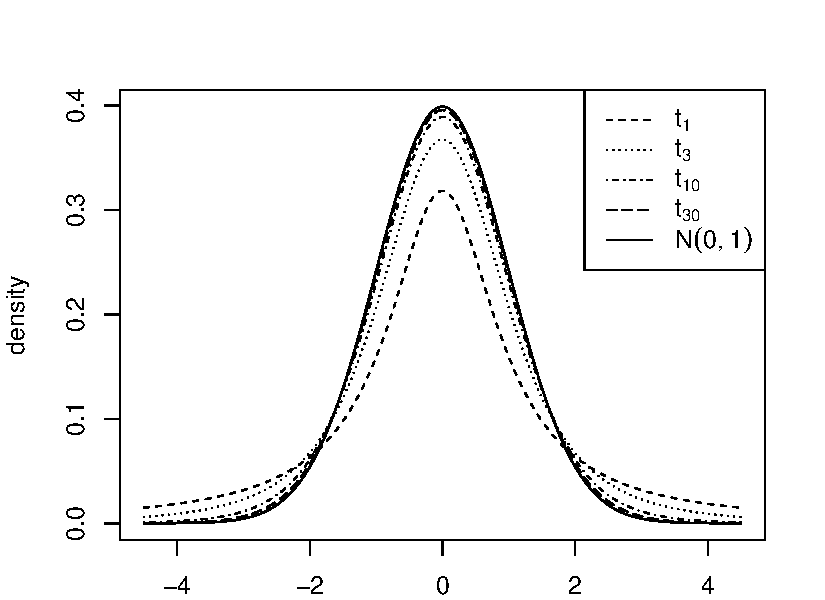
\includegraphics[width=\maxwidth]{figure/unnamed-chunk-1-1} 
\end{knitrout}
\clearpage

\textbf{Remarks}:
\begin{itemize}
\item Similar to the standard normal distribution, the $t$-distribution is bell-curve shaped, symmetric, and centered about zero.
\item Remarkably, the t-score, $t=(\bar{x} - \mu)/(s / \sqrt{n})$ depends on the sample standard deviation $s$, not the population standard deviation $\sigma$; this is one of its most useful properties.
\item The $t$-distribution has wider tails than the standard normal distribution.
\item The $t$-distribution approaches the standard normal distribution as $n$ gets large.  That is, $t_{n-1} \rightarrow N(0,1)$ as $n \rightarrow \infty$.  In fact, when the degrees of freedom is about 30 or more, the $t$-distribution is nearly indistinguishable from the standard normal distribution.\\ %Cite OpenIntro, p.~221
\end{itemize}

\textbf{Ex1}: Simulating random numbers from $t_6$
\begin{knitrout}
\definecolor{shadecolor}{rgb}{0.969, 0.969, 0.969}\color{fgcolor}\begin{kframe}
\begin{alltt}
\hlkwd{set.seed}\hlstd{(}\hlnum{999}\hlstd{)}
\hlstd{t} \hlkwb{<-} \hlkwd{rt}\hlstd{(}\hlnum{5000}\hlstd{,} \hlkwc{df}\hlstd{=}\hlnum{6}\hlstd{)}
\hlkwd{par}\hlstd{(}\hlkwc{mfrow}\hlstd{=}\hlkwd{c}\hlstd{(}\hlnum{1}\hlstd{,}\hlnum{2}\hlstd{),} \hlkwc{cex}\hlstd{=}\hlnum{0.75}\hlstd{)}
\hlkwd{hist}\hlstd{(t)}
\hlkwd{qqnorm}\hlstd{(t)}
\hlkwd{qqline}\hlstd{(t)}
\end{alltt}
\end{kframe}
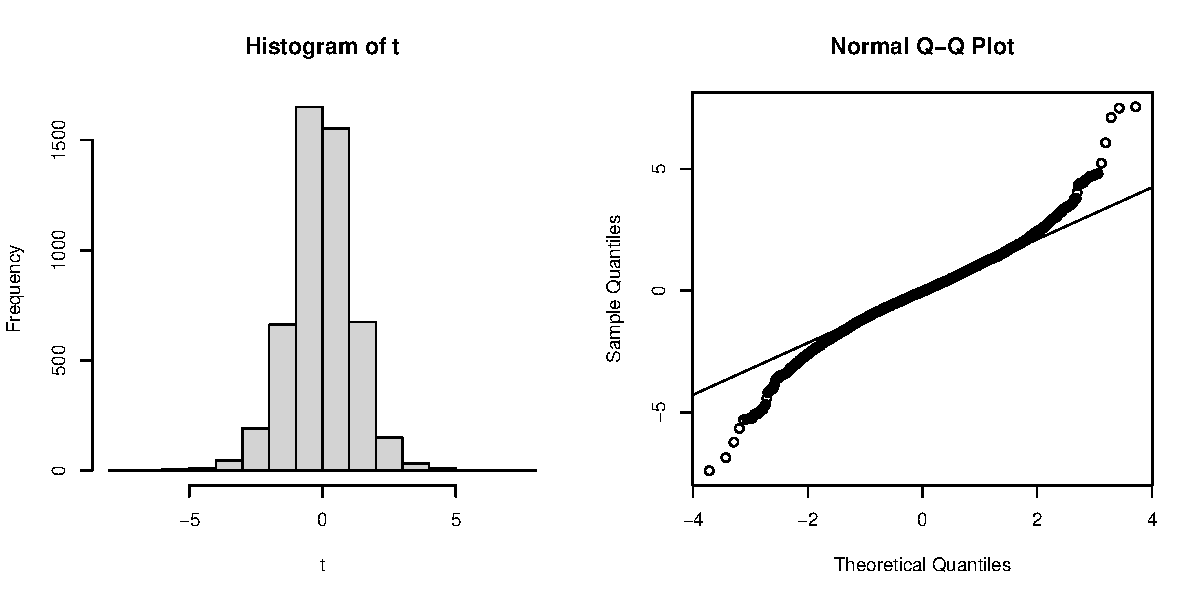
\includegraphics[width=\maxwidth]{figure/unnamed-chunk-2-1} 
\end{knitrout}
\clearpage

\textbf{Constructing a confidence interval for $\mu$ when $\sigma$ is unknown and the population distribution is normal}\\

Let $X_1, X_2, \cdots, X_n$ be a random sample of size $n$ from a normal population distribution;\\ i.e., $X_i \sim N(\mu, \sigma)$.  Since the random variable $\frac{\bar{X} - \mu}{S / \sqrt{n}}$ follows a $t$-distribution with $n-1$ degrees of freedom we can write the following probability statement:
\begin{align*}
P \left( -t_{\alpha/2; n-1} < \frac{\bar{X} - \mu}{S / \sqrt{n}} < t_{\alpha/2; n-1} \right) = 1 - \alpha
\end{align*}

Rearranging terms in the above probability statement gives:
\begin{align*}
P(\bar{X} - t_{\alpha/2; n-1} S / \sqrt{n} < \mu < \bar{X} + t_{\alpha/2; n-1} S / \sqrt{n}) = 1-\alpha
\end{align*}

Therefore, a $100(1-\alpha)$\% confidence interval for $\mu$ is given by
\begin{align*}
\bar{x} \pm t_{\alpha/2; n-1} \frac{s}{\sqrt{n}}
\end{align*}

The critical value $t_{\alpha/2; n-1}$ is defined as follows:

\begin{knitrout}
\definecolor{shadecolor}{rgb}{0.969, 0.969, 0.969}\color{fgcolor}
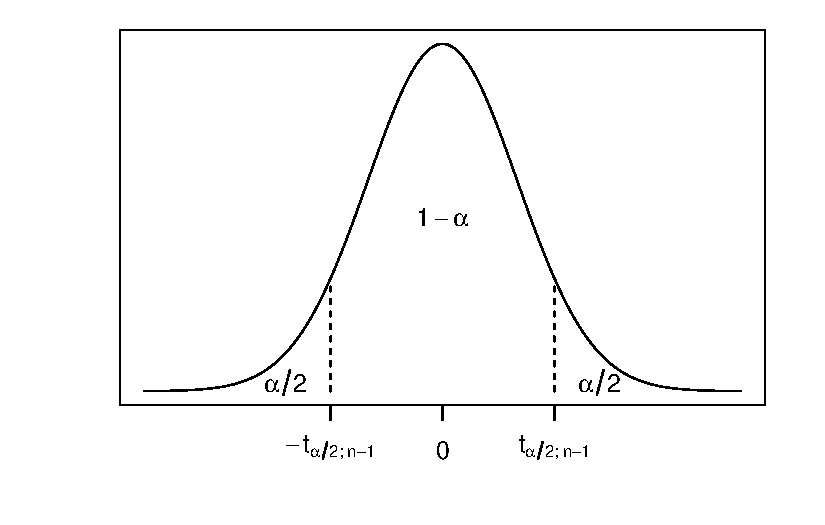
\includegraphics[width=\maxwidth]{figure/unnamed-chunk-3-1} 
\end{knitrout}

In R, $t_{\alpha/2;n-1} = \texttt{qt(1-alpha/2, df=n-1)}$\\



\clearpage

\textbf{Conditions:}  The t-confidence interval for $\mu$ is valid if the following conditions are satisfied:
\begin{itemize}
\item Sample observations are independent.  Generally, this is satisfied when the data come from a random sample.
\item The sample size is large ($n \geq 30$), and there are no extreme outliers.  This implies that the sampling distribution for $\bar{X}$ is approximately normal according to the central limit theorem.
\item Otherwise, if the sample size is small ($n < 30$), the data should follow an approximate normal distribution.  Graphical methods can be used to check this (box plot, histogram, normal QQ plot).
\end{itemize}

\textbf{Remark:}  When the sample size is large ($n \geq 30$), we can use either a $t$ or $z$ critical value to make a confidence interval for $\mu$, since the distributions are nearly identical.\\

% Old notes
% \begin{itemize}
% \item Use the $t$-critical value in the confidence interval for $\mu$ when the sample size is small ($n<30$) and the data are approximately normally distributed.
% \item For large sample sizes ($n \geq 30$) the critical values calculated using the $t$ or $z$ distributions are approximately the same.  Moreover, because of the CLT, we do not need to assume that the population distribution is normal.  
% \item $t$-critical values are larger than corresponding $z$-critical values, so confidence intervals constructed using $t$-critical values are wider.\\
% \end{itemize}

\textbf{Ex2}:  Let $T$ be a random variable following a $t$-distribution with 9 degrees of freedom.
\begin{enumerate}[(a)]
\item Calculate $P(T < 1.5)$\\
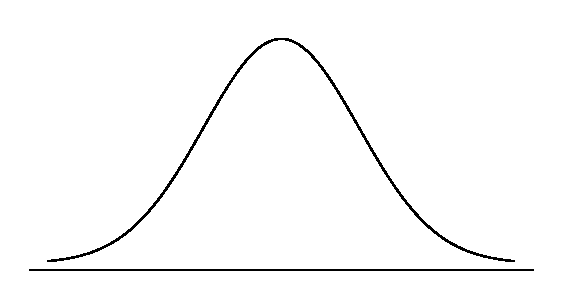
\includegraphics[scale=0.55]{norm_draw.pdf}
\vspace{1cm}



\item Calculate $P(-0.75 < T < 1.5)$\\
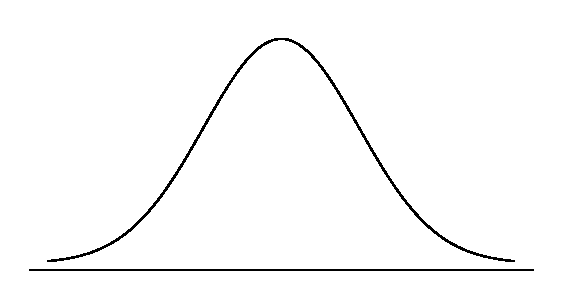
\includegraphics[scale=0.6]{norm_draw.pdf}
\vspace{1cm}

% \medskip
% {\color{blue} $P(-0.75 < T < 1.5) = P(T < 1.5) - P(T < -0.75)$}


\item Find the value $c$ such that $P(T > c) = 0.2$\\
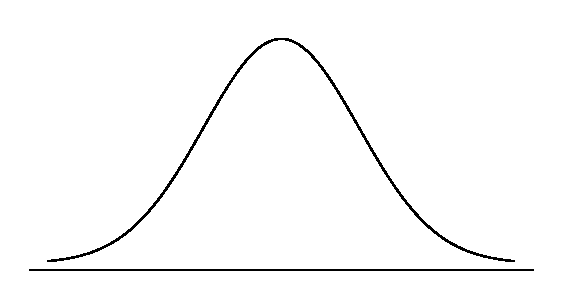
\includegraphics[scale=0.6]{norm_draw.pdf}
\vspace{1cm}

% \medskip
% {\color{blue} $P(T > c) = 0.2 \implies P(T < c) = 0.8$}

\end{enumerate}
\clearpage

\textbf{Ex3}:  Compare the critical values $t_{\alpha/2; n-1}$ and $z_{\alpha/2}$ when the sample size $n=30$ and the confidence level is 0.95.\\
\begin{multicols}{2}
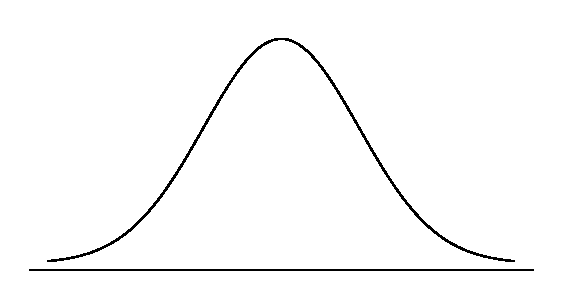
\includegraphics[scale=0.6]{norm_draw.pdf}

\columnbreak

{\color{blue}
$t_{0.025; 29} = \texttt{qt(0.975, df=29)} = 2.045$\\
$z_{0.025} = \texttt{qnorm(0.975)} = 1.96$\\

The critical values are close when $n=30$.\\  
The $t$-critical value is slightly larger.\\
}
\end{multicols}

\bigskip

\textbf{Ex4}:  Below are some summary statistics and a box plot for the ages of a random sample of $n=26$ female athletes who participated in the 2012 Olympic Games in London.  Using this information, calculate and interpret a 95\% confidence interval for the population mean age.  Comment on whether the conditions for the interval appear satisfied.\footnote{Data obtained from the data set \texttt{Olympics2012} in the R package \texttt{resampledata}.} 

\begin{table}[ht]
\begin{tabular}{lllll}
\hline
n & $\bar{x}$ & s & min & max\\
\hline
26 & 26.9 & 4.5 & 19 & 36
\end{tabular}
\end{table}

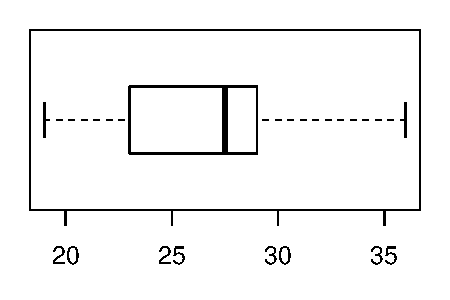
\includegraphics[scale=0.7]{age_boxplot.pdf}

{\color{blue} The conditions for the interval are satisfied:  First, the independence condition is met since the data come from a random sample.  Second, the data follow an approximate normal distribution in the box plot, and there are no outliers (we need to check normality since $n < 30$).\\   

At the $0.95$ confidence level, the critical value is \texttt{qt(0.975, df=25) = 2.06}. Therefore, a 95\% confidence interval for $\mu$ is given by:
$$\bar{x} \pm t_{\alpha / 2; n-1} \frac{s}{\sqrt{n}}
\implies 26.9 \pm 2.06 \cdot \frac{4.5}{\sqrt{26}}
\implies (25.08, 28.72)$$

Interpretation: We are 95\% confident that the population mean age, $\mu$, is between 25.08 and 28.72.
}




\clearpage
\textbf{Simulation Study}:  Compare the coverage of confidence intervals constructed using the $t$ and $z$ distributions when repeatedly taking samples of size $n=5$ from a\\ $N(\mu=50,\sigma=10)$ population distribution.  Use a 95\% confidence level.

\begin{knitrout}
\definecolor{shadecolor}{rgb}{0.969, 0.969, 0.969}\color{fgcolor}\begin{kframe}
\begin{alltt}
\hlkwd{set.seed}\hlstd{(}\hlnum{999}\hlstd{)}
\hlstd{mu} \hlkwb{<-} \hlnum{50}
\hlstd{count_t} \hlkwb{<-} \hlstd{count_z} \hlkwb{<-} \hlnum{0}
\hlkwa{for}\hlstd{(i} \hlkwa{in} \hlnum{1}\hlopt{:}\hlnum{1000}\hlstd{) \{}
  \hlstd{samp} \hlkwb{<-} \hlkwd{rnorm}\hlstd{(}\hlnum{5}\hlstd{,} \hlkwc{mean}\hlstd{=}\hlnum{50}\hlstd{,} \hlkwc{sd}\hlstd{=}\hlnum{10}\hlstd{)}

  \hlcom{# t-interval}
  \hlstd{tcrit} \hlkwb{<-} \hlkwd{qt}\hlstd{(}\hlnum{0.975}\hlstd{,} \hlkwc{df}\hlstd{=}\hlnum{4}\hlstd{)}
  \hlstd{ci_lower} \hlkwb{<-} \hlkwd{mean}\hlstd{(samp)} \hlopt{-} \hlstd{tcrit} \hlopt{*} \hlkwd{sd}\hlstd{(samp)} \hlopt{/} \hlkwd{sqrt}\hlstd{(}\hlnum{5}\hlstd{)}
  \hlstd{ci_upper} \hlkwb{<-} \hlkwd{mean}\hlstd{(samp)} \hlopt{+} \hlstd{tcrit} \hlopt{*} \hlkwd{sd}\hlstd{(samp)} \hlopt{/} \hlkwd{sqrt}\hlstd{(}\hlnum{5}\hlstd{)}
  \hlkwa{if}\hlstd{(mu} \hlopt{>=} \hlstd{ci_lower} \hlopt{&} \hlstd{mu} \hlopt{<=} \hlstd{ci_upper) \{}
    \hlstd{count_t} \hlkwb{<-} \hlstd{count_t} \hlopt{+} \hlnum{1}
  \hlstd{\}}

  \hlcom{# z-interval}
  \hlstd{zcrit} \hlkwb{<-} \hlkwd{qnorm}\hlstd{(}\hlnum{0.975}\hlstd{)}
  \hlstd{ci_lower} \hlkwb{<-} \hlkwd{mean}\hlstd{(samp)} \hlopt{-} \hlstd{zcrit} \hlopt{*} \hlkwd{sd}\hlstd{(samp)} \hlopt{/} \hlkwd{sqrt}\hlstd{(}\hlnum{5}\hlstd{)}
  \hlstd{ci_upper} \hlkwb{<-} \hlkwd{mean}\hlstd{(samp)} \hlopt{+} \hlstd{zcrit} \hlopt{*} \hlkwd{sd}\hlstd{(samp)} \hlopt{/} \hlkwd{sqrt}\hlstd{(}\hlnum{5}\hlstd{)}
  \hlkwa{if}\hlstd{(mu} \hlopt{>=} \hlstd{ci_lower} \hlopt{&} \hlstd{mu} \hlopt{<=} \hlstd{ci_upper) \{}
    \hlstd{count_z} \hlkwb{<-} \hlstd{count_z} \hlopt{+} \hlnum{1}
  \hlstd{\}}
\hlstd{\}}
\hlstd{count_t} \hlopt{/} \hlnum{1000}
\end{alltt}
\begin{verbatim}
## [1] 0.948
\end{verbatim}
\begin{alltt}
\hlstd{count_z} \hlopt{/} \hlnum{1000}
\end{alltt}
\begin{verbatim}
## [1] 0.878
\end{verbatim}
\end{kframe}
\end{knitrout}

Conclusion: The proportion of $t-$confidence intervals that contain $\mu=50$ is 0.948, which is close to the 0.95 confidence level.  However, the proportion of $z-$confidence intervals that contain $\mu=50$ is 0.878, which is less than the 0.95 confidence level (intervals are too narrow).
\clearpage

\end{document}
